\section{La struttura dell'atomo}
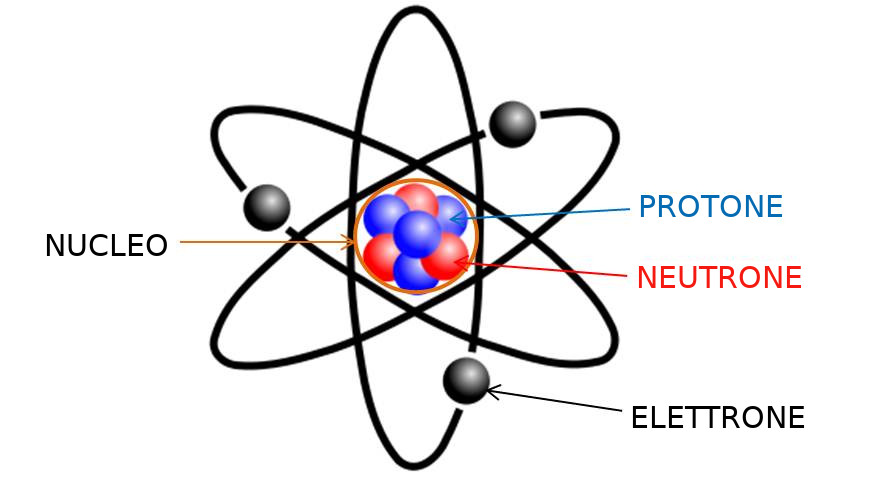
\includegraphics{atom.jpg}
L'atomo  è l'elemento più piccolo della materia ad avere proprietà chimiche. Esso è costituito da tre particelle subatomiche: i protoni e neutroni, che insieme formano il nucleo, e gli elettroni, che orbitano attorno ad esso lungo gli orbitali.

\section{L'uranio e la fissione nucleare}
L'uranio è un metallo pesante poco abbondante, ma largamente diffuso; se viene bombardato da un neutrone il suo nucleo si spezza in due nuclei più leggeri, il bario e il cripto. Da questa reazione, detta fissione nucleare, si libera una notevole quantità di energia e altri neutroni, che vanno a loro volta a colpire altri atomi di uranio. Si tratta di una reazione a catena, che una volta innescata continua da sola, liberando quantità sempre crescenti di energia.

\noindent
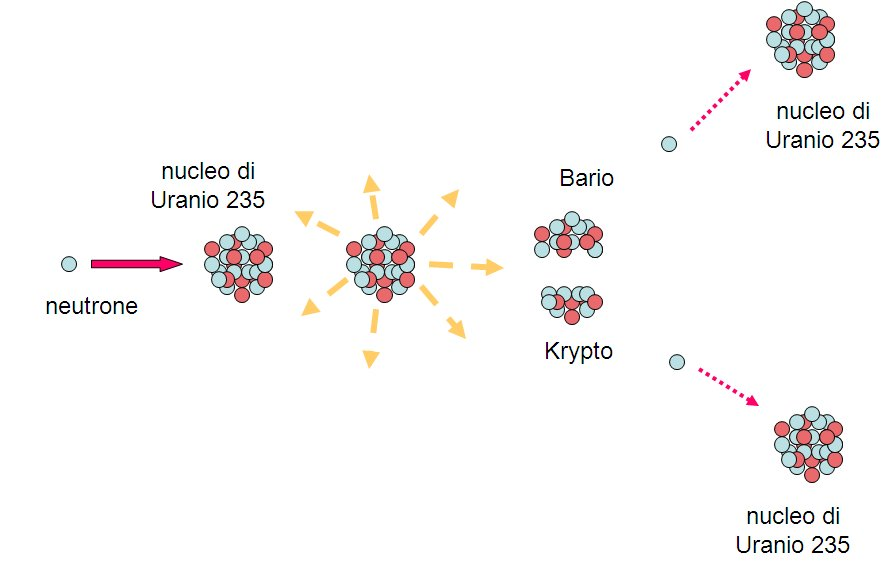
\includegraphics[width=\textwidth]{fissione.jpg}

Il primo dispositivo in grado di fare ciò fu ideato da Fermi ed entrò in funzione a Chicago il 2 dicembre 1942. Tale dispositivo venne chiamato pila atomica o reattore nucleare. E' formato da un'involucro di piombo nel cui interno si trova un cubo di grafite, sostanza che rallenta il movimento dei neutroni; nella grafite sono inserite delle barre di uranio alternate a barre di controllo fatte di boro e di cadmio, sostanze che regolano la quantità di neutroni assorbendoli se sono in eccesso. Sollevando o abbassando le barre di controllo è possibile innescare o bloccare la reazione a catena.
